\documentclass[10pt]{article}
\usepackage[top=1in, bottom=1in, right=1in, left=1in, nohead]{geometry}
\usepackage{amsmath}
\usepackage{graphicx}
\usepackage{amsfonts}
\usepackage{listings}
%%%%%%%%%%%%%%%%%%%%%%%%%%%%%%%%%%%%%%%%%%%
% MATLAB auto-generated code add-ons
\usepackage{color}
\sloppy
\definecolor{lightgray}{gray}{0.5}
\setlength{\parindent}{0pt}
%%%%%%%%%%%%%%%%%%%%%%%%%%%%%%%%%%%%%%%%%%%

\begin{document}

\title{MAE598: Design Optimization Homework 1}
\author{Tanner Bitz}
\maketitle

\section{Problem 1}
\subsection{Problem Statement:}
Using matlab's \textit{fmincon} and Scipy's optimization solvers, optimize the following:

\begin{equation}
\begin{aligned}
	& \underset{x}{\text{min}}
	& & 24.55 x_1 + 26.75 x_2 +39.00 x_3 + 40.50 x_4 \\
	& \text{subject to} 
	& & 2.3 x_1 + 5.6 x_2 + 11.1 x_3 + 1.3 x_4 - 5 \geq 0 \\
	& & & 12 x_1 + 11.9 x_2 + 41.8 x_3 + 52.1 x_4 - 21 - 1.645 {(0.28 {x_1}^2 + 0.19 {x_2}^2 + 20.5 {x_3}^2 + 0.62 {x_4}^2)}^{\frac{1}{2}} \geq 0 \\
	& & & x_1 + x_2 + x_3 + x_4 - 1 = 0 \\ 
	& & & 0 \leq x_i, i = 1, \ldots , 4
\end{aligned}
\end{equation} 

\subsection{Fmincon} 
\textbf{MATLAB code in the 'problem 1' section of 'mae598\_desopt\_hw1\_tannerbitz.m' file.  The nonlinear constraint function is the 'p1\_nonlincon.m' file} \\

Syntax:

\begin{equation*}
	x = \text{fmincon(fun, x0, A, b, Aeq, beq, lb, ub, nonlcon)}
\end{equation*}

\textbf{fun} is the objective function.  It will be an anonymous function of the form: 

\begin{equation*}
	fun = @(x) 24.55*x(1) + 26.75*x(2) + 39.00*x(3) + 40.50*x(4);
\end{equation*}

\textbf{x0} is the intial position

\begin{equation*}
	x0 = [1, 1, 1, 1];
\end{equation*}

\textbf{A, b} are linear ineqality constraints of the form $Ax \leq b$. Of the constraints in the problem, the following are linear inequalities: 

\begin{equation*}
\begin{aligned}
	& 2.3 x_1 + 5.6 x_2 + 11.1 x_3 + 1.3 x_4 - 5 \geq 0 \\
	& 0 \leq x_i, i = 1, \ldots, 4
\end{aligned}
\end{equation*}

Rearranged, these equations become:
\begin{equation*}
\begin{aligned}
	& 2.3 x_1 + 5.6 x_2 + 11.1 x_3 + 1.3 x_4 \geq 5 \\
	& x_i \geq 0, i = 1, \ldots, 4
\end{aligned}
\end{equation*}

Multiply by -1 to flip the equality signs:
\begin{equation*}
\begin{aligned}
	& -2.3 x_1 - 5.6 x_2 - 11.1 x_3 - 1.3 x_4 \leq -5 \\
	& -x_i \leq 0, i = 1, \ldots, 4
\end{aligned}
\end{equation*}

Put into matlab A, and b are:
\begin{equation*}
	A = \begin{bmatrix}
	-2.3 & -5.6 & -11.1 & -1.3 \\
	-1 & 0 & 0 & 0 \\
	0 & -1 & 0 & 0 \\
	0 & 0 & -1 & 0 \\
	0 & 0 & 0 & -1
	\end{bmatrix}
\end{equation*}

\begin{equation*}
	b = {\begin{bmatrix}
	-5 & 0 & 0 & 0 & 0
	\end{bmatrix}}^T
\end{equation*}

\textbf{Aeq, beq} are linear equalities of the form $\text{Aeq} \cdot \text{x = beq}$. Of the constraints from the problem, the following is the only linear equality:

\begin{equation*}
	x_1 + x_2 + x_3 + x_4 -1 = 0
\end{equation*}

Rearranged this is:

\begin{equation*}
	x_1 + x_2 + x_3 + x_4 = 1
\end{equation*}

Aeq and beq now become:

\begin{equation*}
	Aeq = [1, 1, 1, 1];
\end{equation*}

\begin{equation*}
	beq = 1;
\end{equation*}

\textbf{lb, ub} are lower bound and upper bound constraints.  These were not specified in the problem statement so they will be:

\begin{equation*}
\begin{aligned}
	& lb = []; \\
	& ub = []; \\
\end{aligned}
\end{equation*}

\textbf{nonlcon} are nonlinear constraints. They can be an inequality or an equality with the forms:
\begin{equation*}
\begin{aligned}
	& \text{c(x)} \leq 0 \\
	& \text{ceq(x)} = 0 
\end{aligned}
\end{equation*}
The following is the only nonlinear constraint in this problem:

\begin{equation*}
	12 x_1 + 11.9 x_2 + 41.8 x_3 + 52.1 x_4 - 21 - 1.645 {(0.28 {x_1}^2 + 0.19 {x_2}^2 + 20.5 {x_3}^2 + 0.62 {x_4}^2)}^{\frac{1}{2}} \geq 0
\end{equation*}

Multiply by -1 to flip the inequality sign.

\begin{equation*}
	-12 x_1 - 11.9 x_2 - 41.8 x_3 - 52.1 x_4 + 21 + 1.645 {(0.28 {x_1}^2 + 0.19 {x_2}^2 + 20.5 {x_3}^2 + 0.62 {x_4}^2)}^{\frac{1}{2}} \leq 0
\end{equation*}

There is no equality, just an inequality in this problem, so the matlab function will be:

\begin{equation*}
\begin{aligned}
	& \text{function [c, ceq] = nonlincon(x)} \\
	& c = -12*x(1) - 11.9*x(2) - 41.8*x(3) - 52.1*x(4) + 21 + ... \\
	& 1.645*((0.28*x(1)^2 + 0.19*x(2)^2 + 20.5*x(3)^2 + 0.62*x(4)^2)^{(1/2)}; \\
	& \text{ceq = [];} \\
	& \text{end}
\end{aligned}
\end{equation*}

\textbf{Solution: $x = [0.6355, 0.000, 0.3127, 0.0518]$}

\subsection{Scipy Optimization}
\textbf{Python code in the 'problem 1' section of 'mae598\_desopt\_hw1p1\_tannerbitz.py' file.} \\

To solve this optimization problem, I will use the minimize function in the scipy.optimize subpackage.  It's syntax is as follows:

\begin{equation*}
	\text{res = minimize(fun, x0, constraints)}
\end{equation*}

\textbf{fun} is a callable (i.e. a function), which was implemented with a lambda function. (A lambda function is similar to an anonymous function in matlab).

\begin{equation*}
\text{objectivefun = lambda x: 24.55*x[0] + 26.75*x[1] + 39.00*x[2] + 40.50*x[3]}
\end{equation*}

\textbf{x0} is the initial position.  This is implemented with a numpy array of shape (m,). m is 4 in this case. 

\begin{equation*}
	\text{initX = np.array([1, 1, 1, 1])}
\end{equation*}

\textbf{constraints} is a list of dicts with pairs for 'type' and 'fun'. 'type' can either be an 'eq' for equality, and 'ineq' for inequality. 'fun' must be a callable representing a constraint with an assumed form of:

\begin{equation*}
\begin{aligned}
	& f(x) \geq 0 & \text{for inequalities} \\
	& f(x) = 0 & \text{for equalities}
\end{aligned}
\end{equation*}

These constraints can be linear or nonlinear.  A callable was made for each constraint, and the list of dicts was formed:

\begin{equation*}
\begin{aligned}
\text{cons = ([} & \text{{'type': 'ineq', 'fun': linconineq1},} \\
          & \text{{'type': 'ineq', 'fun': linconineq2},} \\
          & \text{{'type': 'ineq', 'fun': linconineq3},} \\
          & \text{{'type': 'ineq', 'fun': linconineq4},} \\
          & \text{{'type': 'ineq', 'fun': linconineq5},} \\
          & \text{{'type': 'eq'  , 'fun': linconeq1  },} \\
          & \text{{'type': 'ineq', 'fun': nonlincon1 }])} 
\end{aligned}
\end{equation*}

The optimization was run with the code:

\begin{equation*}
\text{res = minimize(fun=objectivefun, x0=initX, constraints=cons)}
\end{equation*}

The solution was found to be the same as fmincon.

\textbf{Solution: $x = [0.6355, 0.000, 0.3127, 0.0518]$} 

\section{Problem 2}
\subsection{Problem Statement:}
Design a cylindrical cola can of volume V to minimize material usage. Formulate an optimization problem by the following step: (1) Define design variables and the objective (2) State constraints (3) Discuss assumptions made during modeling. \\

Solve your optimization problme with a realistic cola can volume. Is your optimal solution close to the reality? If not, briefly discuss why (not restricted to engineering considerations). 

\subsection{Problem Formulation}
To simplify this problem, it was assumed that the can would be made out of a sheet of material of uniform thickness. This allowed me formulate the objective function as a minimization of the surface area of the cola can as a function of only the radius of the can, r, and the length (height) of the can, l.  Hence, the optimization variables are r, and l. 

\begin{figure}[h]
\centering
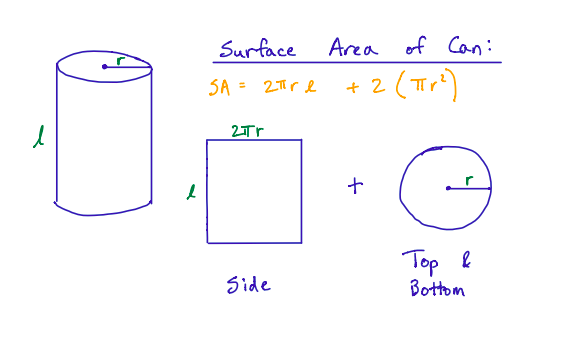
\includegraphics[width=0.8\textwidth]{mae598_desopt_hw1p2_figure.png}
\caption{Surface area of a cola can.}
\end{figure}

The size of a regular cola can is 12 ounces which converts to 354.88 ${cm}^3$.  This volume will become a constraint in optimization problem.  The other constraints are that the radius and the length of the cola can must be positive.

\begin{equation}
\begin{aligned}
	& \text{minimize} & \text{Surface Area} = 2 \pi r l + 2 \pi r^2 \\
	& \text{subject to} & \text{Volume} = \pi r^2 l = 354.88 \\
	& & r \geq 0 \\
	& & l \geq 0 \\ 
\end{aligned}
\end{equation}

\subsection{Solution and Discussion}
\textbf{MATLAB code in the 'problem 2' section of 'mae598\_desopt\_hw1\_tannerbitz.m' file.  The nonlinear constraint function is the 'p2\_nonlincon.m' file} \\

The radius was found to be \textbf{1.51 inches = 3.84cm} and the length was \textbf{3.02 inches = 7.67cm}. \\


The standard size for a can is 4.8 inches tall by 2.1-2.6 inches in diameter.  The optimized version of the can found in this problem is therefore shorter in height and wider in diameter. This makes some sense as a cube is going to have a smaller surface area to volume ratio than a rectangular prism.  This optimization did the analog of that with a cylinder.  It tried to make all dimensions roughly equal (diameter = 3.02 inches and height = 3.02 inches).

\section{Problem 3}
\subsection{Problem Statement}
Consider the problme of grocery shopping with a budget of 30 dollars. you will need 10 units of protein and 20 units of vitamin. You can choose form products A, B, C. the (protein, vitamin) values of them are (5, 0), (0, 6), (3, 2) per unit, and their unit prices are 5, 6, 7 dollar, respoectively. What is the best way to spend your money? Define "best"?

\subsection{Problem Formulation}
I'm going to define the "best" way to spend the money as the least amount of money that allows us to buy a combination of the products that meets our protein and vitamin constraints.  Therefore, our cost function will literally be the cost of shopping trip.

\begin{equation*}
\text{cost} = 5 A + 6 B + 7 C
\end{equation*}

Our constraints will be our protein and vitamin needs.

\begin{equation*}
\begin{aligned}
	 \text{Protein} = & 5 A + 3 C \geq 10 \\
	 \text{Vitamin} = & 6 B + 2 C \geq 20
\end{aligned}
\end{equation*}

And the last constraint we have is the quantities of the products purchased are integers.
\begin{equation*}
\begin{aligned}
& A, B, C \geq 0 \\
& A, B, C \in \mathbb{Z}
\end{aligned}
\end{equation*}

\subsection{Solution and Discussion}
\textbf{MATLAB code in the 'problem 3' section of 'mae598\_desopt\_hw1\_tannerbitz.m' file.} \\

Using MATLAB, it was found that the 30 dollar budget could not be met with integer constraints on the variables.  The optimal integer solution was to buy 2 units of A, 4 units of B, and 0 units of C.  However, this left the total cost at 34, which is greater than our budget. If we weren't to constrain the purchased items to integer values, the optimal solution would be found purchasing 2 units of A, 3.33 units of B, and 0 units of C, for a total cost of 30.  This appears to be the only way to stay within our budget of 30.  

\section{MATLAB Code}
    
    
\subsection*{Contents}

\begin{itemize}
\setlength{\itemsep}{-1ex}
   \item problem 1
   \item problem 2
   \item problem 3
\end{itemize}
\begin{verbatim}
% Tanner Bitz
% MAE 598: Design Optimization
% Fall 2018
% HW 1
\end{verbatim}


\subsection*{problem 1}

\begin{lstlisting}[language=MATLAB]
clear all; clc;
fun = @(x) 24.55*x(1) + 26.75*x(2) + 39.00*x(3) + 40.50*x(4);
x0 = [1,1,1,1];
A = [-2.3, -5.6, -11.1, -1.3;
       -1,    0,     0,    0;
        0,   -1,     0,    0;
        0,    0,    -1,    0;
        0,    0,     0,   -1];

b = [-5, 0, 0, 0 ,0]';
Aeq = [1, 1, 1, 1];
beq = 1;
lb = [];
ub = [];
nonlcon = @p1_nonlincon;
x = fmincon(fun, x0, A, b, Aeq, beq, lb, ub, nonlcon)
\end{lstlisting}

        \color{lightgray} \begin{verbatim}
Local minimum found that satisfies the constraints.

Optimization completed because the objective function is non-decreasing in 
feasible directions, to within the default value of the optimality tolerance,
and constraints are satisfied to within the default value of the constraint tolerance.




x =

    0.6355    0.0000    0.3127    0.0518

\end{verbatim} \color{black}

\begin{lstlisting}[language=MATLAB]
function [c, ceq] = p1_nonlincon(x)
    c = -12*x(1) - 11.9*x(2) - 41.8*x(3) - 52.1*x(4) + 21 + ...
        1.645*(0.28*x(1)^2 + 0.19*x(2)^2 + 20.5*x(3)^2 + 0.62*x(4)^2)^(1/2);
    ceq = [];
end
\end{lstlisting}

\subsection*{problem 2}

\begin{lstlisting}[language=MATLAB]
clear all; clc;
% I am minimizing the surface area of a cyclindrical soda can.
%   x(1) - radius of soda can
%   x(2) - height (or length) of soda can
f = @(x) 2*pi*x(1)*x(2) + 2*pi*x(1)^2;  %minimize surface area
x0 = [1,1];                             %initial guess
A = -eye(2);
b = zeros(1,2);
Aeq = [];
beq = [];
lb = [];
ub = [];
nonlcon = @p2_nonlincon;
x = fmincon(f, x0, A, b, Aeq, beq, lb, ub, nonlcon)
cm2inches = 0.393701;
x_inches = x*cm2inches
\end{lstlisting}

        \color{lightgray} \begin{verbatim}
Local minimum found that satisfies the constraints.

Optimization completed because the objective function is non-decreasing in 
feasible directions, to within the default value of the optimality tolerance,
and constraints are satisfied to within the default value of the constraint tolerance.




x =

    3.8368    7.6736


x_inches =

    1.5105    3.0211

\end{verbatim} \color{black}
    
    
\begin{lstlisting}[language=MATLAB]
function [c, ceq] = p2_nonlincon(x)
    c = [];
    ceq = pi*x(1)^2*x(2) - 354.88;
end

\end{lstlisting}

\subsection*{problem 3}

\begin{lstlisting}[language=MATLAB]
clear all; clc;
% integer programming solution
f = [5, 6, 7]';     % minimizing the total cost given protein/vitamin constraints
intcon = 1:3;       % all variables are integers
A = [-5,  0, -3;
      0, -6, -2;
     -1,  0,  0;
      0, -1,  0;
      0,  0, -1];
b = [-10, -20, 0, 0, 0]';

x = intlinprog(f, intcon, A, b)
integer_optimal_cost = 5*x(1) + 6*x(2) + 7*x(3)

% linear progamming (not integer variable constrained) solution
% A = x(1)
% B = x(2)
% C = x(3)
fun = @(x) 5*x(1) + 6*x(2) + 7*x(3);
x0 = [0, 0, 0]';
y = fmincon(fun, x0, A, b)
optimal_cost = fun(y)
\end{lstlisting}

        \color{lightgray} \begin{verbatim}LP:                Optimal objective value is 30.000000.                                            

Cut Generation:    Applied 2 mir cuts, and 1 strong CG cut.                                         
                   Lower bound is 34.000000.                                                        
                   Relative gap is 0.00%.                                                          


Optimal solution found.

Intlinprog stopped at the root node because the objective value is within a gap
tolerance of the optimal value, options.AbsoluteGapTolerance = 0 (the default
value). The intcon variables are integer within tolerance,
options.IntegerTolerance = 1e-05 (the default value).


x =

    2.0000
    4.0000
         0


integer_optimal_cost =

   34.0000


Local minimum found that satisfies the constraints.

Optimization completed because the objective function is non-decreasing in 
feasible directions, to within the default value of the optimality tolerance,
and constraints are satisfied to within the default value of the constraint tolerance.




y =

    2.0000
    3.3333
    0.0000


optimal_cost =

   30.0000

\end{verbatim} \color{black}


\section{Python Code}

\begin{lstlisting}[language=Python]
import numpy as np
from scipy.optimize import minimize, LinearConstraint, NonlinearConstraint

#MAE 598 Design Optimization - HW1 - Problem 1
objectivefun = lambda x: 24.55*x[0] + 26.75*x[1] + 39.00*x[2] + 40.50*x[3]

# Constraints - Linear Inequalities
def linconineq1(x):
    return 2.3*x[0] + 5.6*x[1] + 11.1*x[2] + 1.3*x[3] - 5

def linconineq2(x):
    return x[0]

def linconineq3(x):
    return x[1]

def linconineq4(x):
    return x[2]

def linconineq5(x):
    return x[3]

# Constraints - Linear Equalities
def linconeq1(x):
    return x[0] + x[1] + x[2] + x[3] -1

# Constraints - Nonlinear Inequalities
def nonlincon1(x):
    return [12*x[0] + 11.9*x[1] + 41.8*x[2] + 52.1*x[3] - 21 -
            1.645*(0.28*x[0]**2 + 0.19*x[1]**2 + 20.5*x[2]**2 + 0.62*x[3]**2)**(1/2)]

cons = ([{'type': 'ineq', 'fun': linconineq1},
         {'type': 'ineq', 'fun': linconineq2},
         {'type': 'ineq', 'fun': linconineq3},
         {'type': 'ineq', 'fun': linconineq4},
         {'type': 'ineq', 'fun': linconineq5},
         {'type': 'eq'  , 'fun': linconeq1  },
         {'type': 'ineq', 'fun': nonlincon1 }])

#Initial condition
initX = np.array([1, 1, 1, 1])

# Perform Optimization
res = minimize(fun=objectivefun, x0=initX, constraints=cons)

# Format and print result
resstring = "{:3.4f}".format(res.x[0])
for i in range(1, len(res.x)):
    resstring += " {:3.4f}".format( float(res.x[i]))

print("The solution to the optimization was: ")
print(resstring)

\end{lstlisting}

\begin{verbatim}
The solution to the optimization was: 
0.6355 0.0000 0.3127 0.0518
\end{verbatim}


\end{document}